% ------------------------------------------------------------------------
% -*-TeX-*- -*-Hard-*- Smart Wrapping
% ------------------------------------------------------------------------
%%% Literature Survey --------------------------------------------------

%\addtolength{\topmargin}{-.875in}
%\addtolength{\textheight}{.875in}
%\footskip
%\nonumchapter{Literature Survey}
%\chapter{Research Approach}
\chapter[Signal Processing and Machine Learning for BCI]{Signal Processing and Machine Learning for Brain-Computer Interfaces}
\label{chap:lit_survey_sig_process}
\epigraph{It is not by trying to improve the candle that we invented electricity.}{--- \textup{Niels Bohr}}
%-------------------------------------------------------------------------
\section{Signal Processing for Cognitive Functions}
%\subsection{Introduction}
%\label{sec:sig_process_intro}
\label{sec:sig_process}
%* Speak of the EEG processing chain that usually consist of signal preprocessing, spatial filtering, classification.
Brain-computer interfaces translate brain signals into control or communication signal; the signal processing and machine learning component is therefore fundamental.
The usual steps in the translation of brain signals consist of signal preprocessing, feature extraction, and finally a feature classification (or regression).

Signal preprocessing is fundamentally a cleaning up of data. 
The operations involved vary depending on the authors. 
They are usually generic operations such as epoching and removal of non-EEG signal added during the recording. 
\cite{bashashati_survey_2007} report on techniques used to this end.

Feature extraction aims at identifying the characteristics in the EEG signals that bear relevant information for the classification task. 
Thus, it plays an important role in the design and choice of appropriate classifiers. 
The performance of BCI depends as much on the features used as on the classifier.
Feature extraction techniques are a set of operations or transformations applied on the raw EEG such that the neurological phenomenon induced by the BCI task is either enhanced or adequately represented. 
From the EEG signal they can extract:
\begin{itemize}
\item  time features e.g. EEG signal amplitudes, signal power \citep{rivet_xdawn_2009},
\item frequency features e.g. band power, power spectral density \citep{bhattacharyya_performance_2010}, 
\item parametric features e.g. Auto Regressive (AR) and adaptive AR (ARR) parameters \citep{zhang_classification_2015}, 
\item time-frequency features e.g. wavelet transforms \citep{kumar_design_2010, dingyin_feature_2011, zhang_comparison_2015}, short-time Fourier transform \citep{kumar_design_2010}, empirical mode decomposition \citep{gaur_empirical_2015, wang_motor_2011,liu_novel_2011}, 
 \item spatial features e.g. Independent Component Analysis (ICA) \citep{wang_enhancing_2006, wang_improving_2013, brunner_spatial_2007}, Common Spatial Patterns (CSP) \citep{ang_filter_2012, barachant_common_2010, blankertz_optimizing_2008}, Canonical Correlation Analysis (CCA) \citep{nakanishi_high-speed_2014, kalunga_ssvep_2013}, Principal Component Analysis (PCA) \citep{kottaimalai_eeg_2013, yu_analysis_2014}, xDAWN \citep{rivet_xdawn_2009}.
\end{itemize}
Detailed reviews of classic feature extraction methods can be found in \citep{lotte_review_2007, nicolas-alonso_brain_2012, bashashati_survey_2007, khorshidtalab_eeg_2011, krusienski_critical_2011}. 
The choice of feature extraction techniques is guided by the neurological phenomenon used in the BCI.
For instance, in SSVEP, relevant information will be contained in the spectral features while in P300, temporal features will suffice. 
\cite{fukunaga_introduction_1990} defines feature extraction for classification as a search, among all possible singular transformations, for the best subspace which preserves class separability as much as possible in the lowest possible dimensional space.

Spatial filters (from which spatial features are extracted) have proven to be successful tools in extracting (or enhancing) the neurological phenomenon from the EEG signal. 
The information of interest is hidden in the recorded EEG, a mixture of simultaneous active brain sources and noise sources in the recording environment. 
The signal of interest could be overlapped in time, space, and frequency with multiple signals. 
Using \textit{a priori} knowledge on the phenomenon of interest 
%(\textit{i.e.} unsupervised methods)
 or knowledge deduced from pre-recorded data, spatial filters extract better signal features that make subsequent processing tractable. 
Supervised and semi-supervised approaches lead to highest classification performances.
Once a spatial filter has been applied to EEG data, any feature extraction technique can further be used merely for feature representation. 
%Their effect is trivialised by the spatial filter.

With relevant features, standard classification algorithms such as Linear Discriminant Analysis (LDA) and Support Vector Machine (SVM) \citep{rivet_xdawn_2009, pfurtscheller_self-paced_2010, spuler_one_2012}, Artificial Neural Networks \citep{haselsteiner_using_2000, sturm_interpretable_2016}, Quadratic Discriminant Analysis \citep{friedman_regularized_1989, bhattacharyya_performance_2010}, Hidden Markov Model \citep{obermaier_hidden_2001, lee_pca+hmm+svm_2003, yan_classifying_2008}, and nearest neighbour \citep{cincotti_comparison_2003, schlogl_characterization_2005, bhattacharyya_performance_2010} can be applied.

The signal processing pipeline can be represented as in Figure \ref{fig:processing_pipeline}. 
Removing the preprocessing and the feature representation phases that do not require training, the machine learning pipeline of most successful BCI systems \citep{ang_filter_2012, spuler_one_2012, rivet_xdawn_2009} consists mainly of spatial filtering and classification/regression blocks.

\begin{figure}[!h]
\centering

\includegraphics[width=0.8\columnwidth]{Figures/processing_pipeline}
\caption{BCI signal processing pipeline. The fundamental blocks for machine learning are in blue (\textit{i.e.} spatial filtering and classification). Filters and classifiers are learned from training data. Gray blocks (\textit{i.e.} preprocessing and feature representation) do not require learning. }
\label{fig:processing_pipeline}
\end{figure}
Spatial filters and classifiers are trained offline on pre-recorded data. 
The best preprocessing and feature representation can be chosen based on the offline analysis through cross validation. 

Hereafter, classical couplings of spatial filters and classifiers are illustrated as they are used in machine learning of various BCI types \textit{i.e.} motor imagery, P300, and SSVEP.   

Filtering is based on a modelling of EEG as a linear mixture of multiple neural ensembles to which noise is added:
\begin{equation}
\X = AS+R
\label{eq:eeg_model}
\end{equation} 
where $\X \in \Re^{\dc \times \dt}$ is the EEG recorded on $\dc$ channels over $\dt$ samples, $S \in R^{K \times \dt}$ are the brain sources, $A \in \Re^{\dc \times K}$ is a matrix defining the mixture of the brain sources, and $R \in \Re^{\dc \times \dt}$ is the additive noise, with $\dc \leq K$.  
Spatial filters are designed to extract signal of interest \eqref{eq:eeg_model} based on \textit{a priori} knowledge on the neurological phenomenon of interest or knowledge deduced from pre-recorded data.

%* In each method provide: Brief expllanation, Equations, graphical example (if possible), example of applications (+progress) in BCI
%* Organise these methods per BCI type (ERD, ERP, SSVEP)
%- ICA
%- PCA
%
%I. ERD-ERS (MI)
%- CSP, SVM, LDA, ANN
%II. ERP
%- xDawn
%III. SSVEP
%- CCA, SVM, LDA, ANN
%
%- SVM 
%- LDA
%- ANN
%

\subsection{Motor Imagery Processing} % (ERD/ERS based BCI)}
\label{subsec:sign_proc_mi}
%CSP/LDA
Common Spatial Patterns are spatial filters that has been particularly designed for motor imagery tasks classification \citep{koles_spatial_1990}. 
CSP extracts EEG spatial components that are common to two imagery tasks, but maximising the variance of the signal recorded during one task while minimising the variance in the other task.
The distribution of filtered samples belonging to one imagery task has maximal variance, while the distribution of samples in the other task has minimal variance, or vice-versa as illustrated in Figure \ref{fig:class_scatter_csp}. 
CSP should capture the contralateral effect of ERS versus ERD induced by motor imagery tasks. 

CSP has been successfully coupled with linear discriminant analysis classifiers \citep{dornhege_increase_2004, popescu_single_2007}. 
Indeed like CSP, LDA also relies on data class scatter. 
LDA projects samples into a space where the within-class covariance matrices are minimised, while the between-class covariance matrix is maximised. Here the covariance matrices are proportional to the class scatter.  

\subsubsection{Common Spatial Patterns}

CSP model is given by:
\begin{equation}
\label{eq:csp}
S = WX
\end{equation}
%Given the model given in equation \eqref{eq:eeg_model}, 
CSP finds the filter $W \in \Re^{\dc \times \dc}$ that minimises the variance of the filtered signal $S$ in one condition and maximises it in the other.
\begin{figure}[h!]
\centering
\subfigure[]{
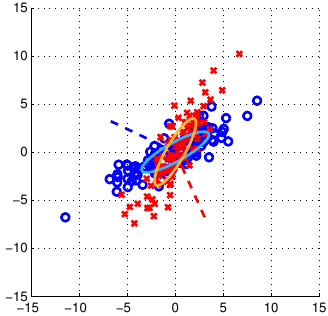
\includegraphics[width=0.4\textwidth]{Figures/class_scatter_before_csp}
\label{fig:class_scatter_before_csp}
}
\subfigure[]{
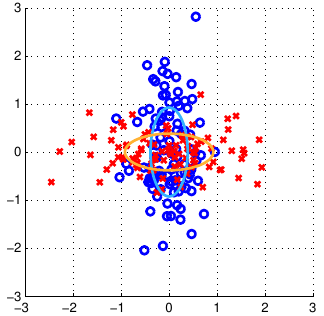
\includegraphics[width=0.4\textwidth]{Figures/class_scatter_after_csp}
\label{fig:class_scatter_after_csp}
}
\caption{CSP effect on class distribution. 
CSP is applied on a 2D toy data set containing samples from two classes marked with red crosses and blue circles. 
(a) Samples distribution is shown before CSP filtering. The ellipses show estimates of each class covariance. 
It can be seen that the two classes are highly correlated. 
The dashed lines show the direction of the CSP projections $\mathbf{w}_j$ ($j=1,2$). 
(b) Distributions after CSP projections. The two distributions are orthogonal, showing that the two classes are uncorrelated. 
Each axis gives the largest variance in one class and the smallest in the other. \citep[Image from][]{blankertz_optimizing_2008}.} 
\label{fig:class_scatter_csp}
\end{figure}
Neglecting additive noise in Equation~\eqref{eq:eeg_model}, the CSP model is equivalent to finding the inverse of $A$:
$W = A^{-1}$. 
In EEG modelling, $A$ is called the \emph{forward model} or the \emph{mixing matrix} and $W$ the \emph{reverse model} or \emph{de-mixing matrix}.  
$A$ describes the spatial pattern. 

Let $\X_i \in \Re^{\dc\times \dt}$ be a band-pass filtered signal of EEG recorded at epoch $i$.
An estimate of its covariance matrix $\cov{i} \in \Re^{\dc\times \dc}$ can be computed as:
\begin{equation}
\label{eq:covmat1}
\cov{i} = \frac{\X_i \X_i^{T}}{trace(\X_i \X_i^{T})} 
\end{equation} 
A class covariance matrix is obtained as: 
\begin{equation}
\cov{(c)} = \frac{1}{N_c} \sum_{i=1}^{N_c} \cov{i}
\end{equation}  
In a two imagery task, $c \in \left\lbrace +,- \right\rbrace$, and $N_c$ is the number of epochs in class $c$. 
\\CSP solves the following problem:

\begin{equation}
\label{eq:csp_problem}
\begin{aligned}
& \underset{W}{\text{maximise}}
& & \mathrm{trace}(W^T \cov{(+)} W) \\
& \text{subject to}
& & W^T(\cov{(+)} + \cov{(-)})W=\eye.
\end{aligned}
\end{equation} 
\begin{figure*}[!th]
    \centering
    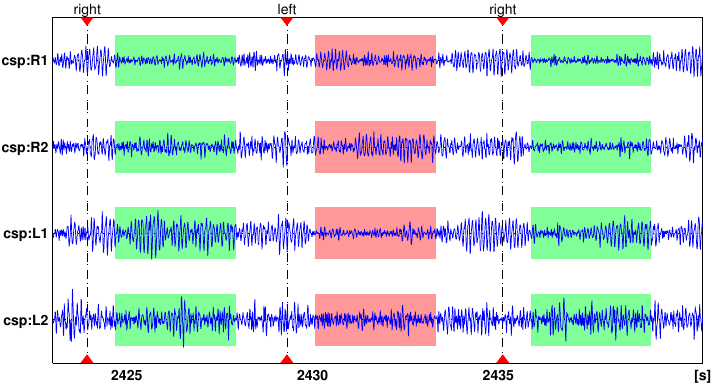
\includegraphics[width=0.8\columnwidth]{Figures/csp_effect}
    \caption{\footnotesize{Effect of CSP filtering. A continuous EEG signal containing two right-hand imagery epochs and one left-hand imagery is filtered using four CSP filters ($\mathbf{w}_j$): csp:R1, csp:R2, csp:L1, and csp:L2. The resulting signals from csp:R1 and csp:R2 have large variance during left hand imagery, while signals from csp:L1 and csp:L2 have large variance during right hand imagery. \citep[Image from][]{blankertz_optimizing_2008}.} }
    \label{fig:csp_effect}
\end{figure*}
The constraint in \eqref{eq:csp_problem}, where $\eye$ is the identity matrix, forces $W^T \cov{(-)} W$ to be minimal when $W^T \cov{(+)} W$ is maximal. 
There are many ways of solving this problem. A simple way is to solve it as a generalised eigenvalue problem \citep{koles_spatial_1990, blankertz_optimizing_2008}:
\begin{equation}
\label{eq:csp_gen_eigen}
\cov{(+)} \mathbf{w}= \lambda \cov{(-)} \mathbf{w} \, ,
\end{equation}
where $\mathbf{w}_j$ ($j=1, \dots, \dc$) are the generalised eigenvectors that constitute the vectors of the matrix $W$, and $\lambda_j = \lambda_j^{(+)}/\lambda_j^{(-)}$, with $\lambda_j^{(c)} = \mathbf{w}_j^T \cov{(c)}\mathbf{w}_j$ where $0 \leq \lambda_j^{(c)} \leq 1$ and $\lambda_j^{(+)} + \lambda_j^{(-)} = 1$. 
$\lambda_j^{(c)}$ is the variance in the filtered signal $\mathbf{s}_j = \mathbf{w}_j^T X$ in the epochs corresponding to class $(c)$.
Thus filtering (\textit{i.e.} projecting) the EEG signal $X_i$ with $\mathbf{w}_j$ that corresponds to the largest $\lambda_ j^{(+)} \rightarrow 1 $, will maximise the variance in class $(+)$ while minimising it in class $(-)$ as illustrated in Figures \ref{fig:csp_effect} and \ref{fig:class_scatter_csp}.

This discussion of CSP is limited to two-class motor imagery. The application of CSP has been extended to multi-class cases \citep{dornhege_increase_2004, grosse-wentrup_multiclass_2008}.

\subsubsection{Linear Discriminant Analysis}

Given a set of $n$ $\dc$-dimensional samples $\x_1, \x_2, \dots, \x_n$ ($\x_i \in \Re^\dc$) , LDA finds a lower dimensional space (typically $\dc-1$) where the data are the most separable.
In a two-class case ($c \in \left\lbrace +, - \right\rbrace$), $n_{(+)}$ samples belong to the positive subset $\mathcal{X}^{(+)}$,
and $n_{(-)}$ samples belong to the negative subset $\mathcal{X}^{(-)}$
LDA finds a projection vector $\w$ that will achieve the mapping
\begin{equation}
y = \w^T \x
\end{equation}
that obtains the $n$ $(\dc-1)$-dimensional samples $y_1, \dots, \y_n$ ($y_i \in \Re^{d-1}$), where the positive subset of the projected data $\mathcal{Y}^{(+)}$ is separable from the negative subset $\mathcal{Y}^{(-)}$.
If the original $\dc$-dimensional samples are highly overlapped, not even the best $\w$ could separate them in a lower dimension. 
A successful application of CSP will avoid such problems.

For separability brings the idea of distance between subsets,
LDA uses the difference of projected samples means:

\[ |\tilde{\m}_{(+)} - \tilde{\m}_{(-)} | \] 
If $\m_{(c)}$ is the $\dc$-dimensional class mean,
\begin{equation}
\label{eq:lda-class-orig-mean}
\m_c = \frac{1}{n_{(c)}} \sum_{\x \in \Xc^{(c)}} \x,
\end{equation}
$\tilde{\m}_{(c)}$ is the mean of projected samples belonging to $\Yc^{(c)}$ and is given by  
%\begin{equation}
%\tilde{\m}_c = \frac{1}{n_{(c)}} \sum_{y \in \mathcal{Y}^{(c)}} y
%\end{equation}
\begin{equation}
\label{eq:lda-class-proj-mean}
  \begin{split}
    \tilde{\m}_{(c)} & = \frac{1}{n_{(c)}} \sum_{y \in \Yc^{(c)}} y
		\\
    & = \frac{1}{n_{(c)}} \sum_{y \in \Yc^{(c)}} \w^T \x = \w^T \m_c ,
  \end{split}  
\end{equation}
Maximising the distance between class means does not ensure class separability. 
If both subset are very scattered, their samples can still be highly overlapped even when their respective means are very distant.
This introduces a second criterion in LDA: the distance between class means should be large relative to the \emph{within-class scatter} given by:
\begin{equation}
\label{eq:lda-within-class-scatter}
\scat_{(c)} = \sum_{y \in \Yc^{(c)}} (y-\tilde{\m}_{(c)})^2  
\end{equation} 
The total within-class scatter is $\scat_{(+)}+\scat_{(-)}$.
LDA uses the function $\w^T \x$ with the vector $\w$ that maximises the criteria 
\begin{equation}
\label{eq:lda-criteria}
J(\w) = \frac{|\tilde{\m}_{(+)} - \tilde{\m}_{(-)} |^2}{\scat_{(+)}+\scat_{(-)}}
\end{equation}
Figure \ref{fig:lda} illustrates a projection of data verifying this criterion. 
\begin{figure*}[!ht]
    \centering
    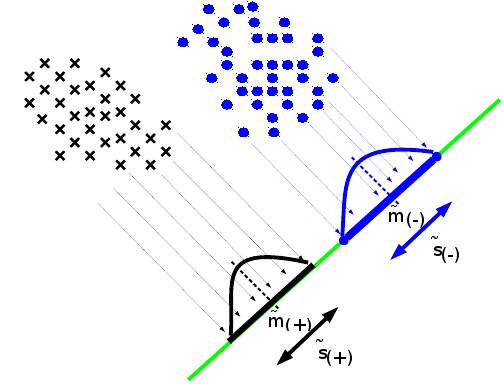
\includegraphics[width=0.5\columnwidth]{Figures/lda}
    \caption{\footnotesize{LDA mapping. The distance $|\tilde{\m}_{(+)}-\tilde{\m}_{(+)}|$} is maximised relative to class variance such as the separability is maximised ($J(\w)$) }
    \label{fig:lda}
\end{figure*}
To express $J(\w)$ in terms of $\w$ and the d-dimensional observed samples, \eqref{eq:lda-class-proj-mean} and \eqref{eq:lda-within-class-scatter} are inserted into \eqref{eq:lda-criteria}, which yields
\begin{equation}
\label{eq:lda-criteria2}
J(\w) = \frac{\w^T \Scat_B \w}{\w^T \Scat_W \w},
\end{equation}
where 
\begin{equation}
\label{lda-b-scatter}
\Scat_B = (\m_{(+)}-\m_{(-)})(\m_{(+)}-\m_{(-)})^T
\end{equation}
is the \emph{between-class scatter matrix}, and 
\begin{equation}
\label{lda-w-scatter}
\Scat_W = \sum_{\x \in \Xc^{(c)}}(\x-\m_{(c)})(\x-\m_{(c)})^T
\end{equation}
is the \emph{within-class scatter matrix}.

Equation \ref{eq:lda-criteria2} is a generalised Rayleigh quotient and can be solved for $\w$ as a generalised eigenvalue problem \citep{duda_pattern_2001}. 

Quadratic Discriminant Analysis (QDA) is a generalisation of LDA to nonlinear boundaries (\textit{i.e.} conic section). 
Unlike LDA, QDA allows different class covariance in the projected space. QDA has also been used for classification of motor imagery tasks \citep{bhattacharyya_performance_2010}. Figure \ref{fig:lda-qda} illustrates the significance of QDA over LDA. 
\begin{figure}[h!]
\centering
\subfigure[]{
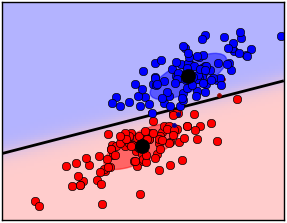
\includegraphics[width=0.4\textwidth]{Figures/lda-separate-data}
\label{fig:lda-separate-data}
}
\subfigure[]{
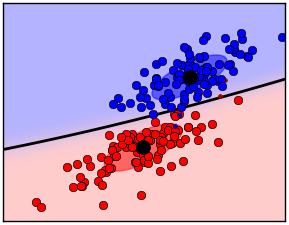
\includegraphics[width=0.4\textwidth]{Figures/qda-separate-data}
\label{fig:qda-separate-data}
}
\subfigure[]{
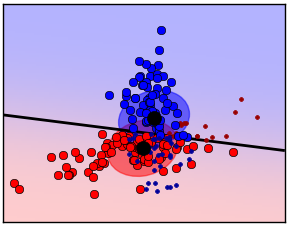
\includegraphics[width=0.4\textwidth]{Figures/lda-overlap-data}
\label{fig:lda-overlap-data}
}
\subfigure[]{
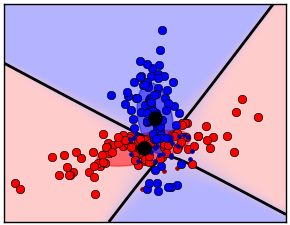
\includegraphics[width=0.4\textwidth]{Figures/qda-overlap-data}
\label{fig:qda-overlap-data}
}
\caption{QDA versus LDA.
Data from two subsets shows with red and blue circles are classified with either LDA (in (a) and (c)) or QDA (in (b) and (d)). The black lines show the classifier separation line. Wrongly classified data are shown with squares instead of circles. 
Class covariances are shown with ellipses of corresponding colours. 
In (a) and (b), the two subsets have similar covariance, while in (c) and (d) they have different covariance \citep{scikit-learn}}
\label{fig:lda-qda}
\end{figure}

%($\x_i \in \Re^d$)

\subsection{SSVEP Processing}% (VEP besed BCI)}
\label{subsec:sign_proc_ssvep}
%CCA + SVM 
Canonical Correlation Analysis (CCA) was recently introduced to classification of SSVEP signal \citep{lin_frequency_2006}. 
It has since been used in the most successful SSVEP-based BCI \citep{bin_online_2009, nakanishi_high-speed_2014}.
It is known that flickering visual stimuli induced an SSVEP that is correlated to the stimuli, \textit{i.e.} the phase and frequency of the signal of interest are known. 
Using this information about the signal of interest, CCA will extract the EEG spatial components that correlate the most with the SSVEP stimuli.
When used as spatial filters, CCA works well when coupled with Support Vector Machine (SVM) classifiers \citep{spuler_one_2012, kalunga_ssvep_2013}.  

\subsubsection{Canonical Correlation Analysis}
\label{subsubsec:cca}
Let  $Y \in \Re^{H \times \dt}$ be a multivariate signal representing the stimulation signal used in recording the EEG signal $\X$.
Per SSVEP principle, $\X$ is expected to be correlated to $Y$. 
Thus CCA will find two projection directions $\w_\X$ and $\w_Y$ such that $\w_X^T \X$ and $\w_Y Y$ have maximal correlation.
$\w_{\X}$ and $\w_Y$ maximises the correlation function $\rho(\w_\X,\w_Y)$:
%In other words, it find the space where the SSVEP -which is correlated to $\Y$, is more observable.
\begin{equation}
\label{eq:cca-rho}
  \begin{split}
    \rho(\w_X,\w_Y) & = \mathrm{corr}(\w_X^T \X,\w_Y Y)
		\\
    & = \frac{\w_{\X}^T \Scat_{\X Y} \w_Y}{\sqrt{\w_{\X}^T \Scat_{\X} \w_X  \w_Y^T \Scat_{Y} \w_Y}},
  \end{split}  
\end{equation}
where $\Scat_{\X Y}$ is the between-set covariance matrix; $\Scat_{\X}$ and $\Scat_{Y}$ are the within-set covariance matrices.
CCA can be solved \citep[as in][]{hardoon_canonical_2004}:
\begin{equation*}
\begin{aligned}
& \underset{\w_X, \w_Y}{\text{maximise}}
& & \w_{\X}^T \Scat_{\X Y} \w_Y \\
& \text{subject to}
& & \w_{\X}^T \Scat_{\X} \w_X = 1, \\
&&& \w_Y^T \Scat_{Y} \w_Y = 1.
\end{aligned}
\end{equation*}
A common way of generating the representation of the simulation signal at frequency $f$ is:
\begin{equation} \label{eq:ref-sig}
    Y_f=\left[
    \begin{array}{c}
    \sin(2\pi f) \\ \cos(2\pi f n) \\
    \vdots \\ \sin(2\pi N_h f n) \\ \cos(2\pi N_h f n)
    \end{array}
    \right],n = \frac{1}{fs}, \frac{2}{fs}, \dots, \frac{\dt}{fs}
\end{equation}  
Where $f_s$ is the EEG sampling frequency, $N_h$ is the number of harmonics, and  $\dt$ the number of sampling points.
$N_h$ is a parameter that can be defined by cross validation.

\subsubsection{Support Vector Machine}
\label{subsubsec:svm}

Support Vector Machines (SVM) have been successfully used in classification of SSVEP signal, and in BCI in general.
The binary SVM decision function is of the form:

\begin{equation}
\label{eq:svm_fct}
y = f(x) = sgn \left( \sum_{i=1}^m y_i \alpha_i k(\x,\x_i) + b \right), y \in \{\pm 1\}
\end{equation}
where $\x$ is the sample variable, $x_i$ a sample in the training data with the label $y_i \in \{\pm 1\}$. $m$ is the number of data samples in the training set, $\alpha_i$ the weight of sample $x_i$ and $b$ an offset.
$k(\cdot,\cdot)$ is a kernel, \textit{i.e.} a function that returns a real number characterising the similarity between its inputs. 
In a Euclidean space, the dot product would often be used as a linear kernel \eqref{eq:linear-kernel}.
Function \eqref{eq:svm_fct} defines a hyperplane of decision boundary that separates samples in the negative class from samples in the positive class.
SVM ignores the influence of training samples $x_i$ that are very far away from the decision boundary by setting their corresponding weight $\alpha_i$ to zero.
Thus, it only relies on a subset of data close to the decision boundary. They are called \emph{Support Vectors}. 
This reduces model complexity and improves generalisation.  
Thought there could possibly exist many hyperplanes that accurately separate data into their specific classes, SVM finds the unique hyperplane that has maximum margin of separation between the support vectors and itself. 
This fact gives SVM classifiers good generalisation performance and robustness to overfitting \citep{scholkopf_learning_2001, ang_filter_2008, ang_filter_2012}. 
To find such a hyperplane SVM solves the following problem:

\begin{equation}
\label{eq:svm_problem}
\begin{aligned}
& \underset{\w \in \dotSpace, b \in \Re}{\text{minimise}}
& & \frac{1}{2} \w^T \w \\
& \text{subject to}
& & y_i( \left\langle \x_i, \w \right\rangle + b )\geq 1, i = 1, \dots, m.
\end{aligned}
\end{equation} 
where $\dotSpace$ is a dot product space, and $m$ is the number of training samples.

\begin{figure}[!h]
\centering
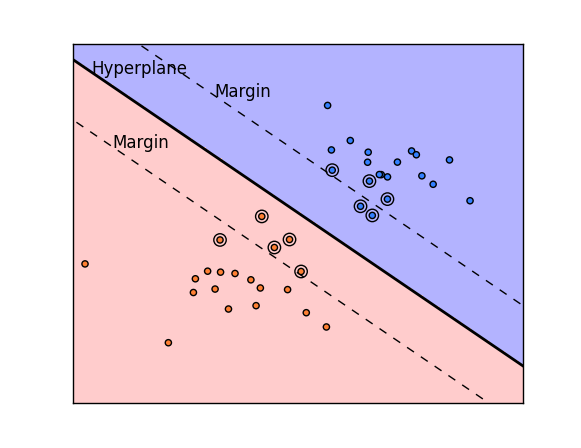
\includegraphics[width=0.8\columnwidth]{Figures/svm}
\caption{Examples of SVM classifiers. 
SVM is applied on 2D artificial data forming two classes represented in red and blue. The hyperplane $\left\langle \x_i, \w \right\rangle + b = 0$ separating the two classes is shown, as well as the margins$\left\langle \x_i, \w \right\rangle + b \geq \frac{1}{||\w||}$. Only few samples relatively close to the hyperplanes are used as support vectors; they are shown with big circles \citep{scikit-learn}.}
\label{fig:svm}
\end{figure}
To achieve nonlinear classification SVM uses kernels other than the dot product.
Such kernels are needed in cases where (1) features are better separated in a higher-dimensional space, (2) features are defined in a space where the dot product is not defined, or (3) the separating line is not linear.
Since SVM is based on the dot product (Eq. \eqref{eq:svm_problem}), the kernel used in the input space $\inputSpace$ corresponds to dot product in $\dotSpace$ via a mapping $\Phi$,

\begin{equation}
\label{eq:kernel-phi}
  \begin{split}
    \Phi : & \inputSpace \rightarrow \dotSpace
		\\
    		   & x \rightarrow \mathbf{\x} := \Phi(x),
  \end{split}  
\end{equation}
such that,
\begin{equation}
\label{eq:kernel-phi2}
k(x,x^{\prime}) = \left\langle \Phi(x), \Phi(x^{\prime}) \right\rangle .
\end{equation}
Examples of such kernels admitting the representation of the form \eqref{eq:kernel-phi} that are often used in SVM are the linear kernel (\textit{i.e.} dot product), the polynomial kernel, and the radial basis function (RBF) kernel.

\begin{figure}[h!]
\centering
\subfigure[]{
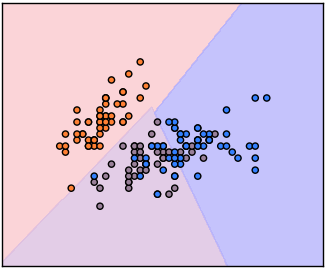
\includegraphics[width=0.3\textwidth]{Figures/svm-linear-kernel}
\label{fig:svm-linear-kernel}
}
\subfigure[]{
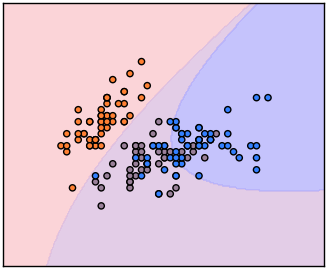
\includegraphics[width=0.3\textwidth]{Figures/svm-poly-kernel}
\label{fig:svm-poly-kernel}
}
\subfigure[]{
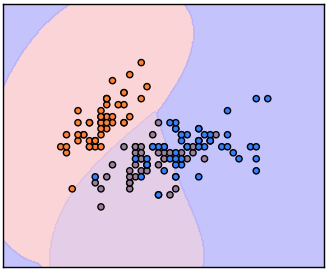
\includegraphics[width=0.3\textwidth]{Figures/svm-rbf-kernel}
\label{fig:svm-rbf-kernel}
}
\caption{Multiclass SVM classification with different kernels on 2D projection of the iris dataset. The decision surface separating three classes are shown. The x-axis and y-axis represent sepal length and sepal width respectively. (a) Linear kernel, (b) polynomial kernel of order 3, (c) RBF kernel \citep{scikit-learn}.}
\label{fig:svm-kernels}
\end{figure}
\emph{Linear kernel}:\\
\begin{equation}
\label{eq:linear-kernel}
k(\x_1,\x_2) = \left\langle \x_1, \x_2 \right\rangle = \x_1^T \x_2.
\end{equation} 
\emph{Polynomial kernels}:\\
\begin{equation}
\label{eq:poly-kernel}
k(x,x^{\prime}) = \left\langle x,x^{\prime} \right\rangle^d, 
\end{equation}
where $d$ is the polynomial degree.\\
\emph{Radial basis function (RBF) kernels}:\\
\begin{equation}
\label{eq:rbf-kernel}
k(x,x^{\prime}) = \exp(- ||x-x^{\prime}||^2), 
\end{equation}
Details on various implementations of SVM classifiers can be found in \citep{chang_libsvm:_2011}

\subsection{P300 Processing}% (ERP-based BCI)}
\label{subsec:sign_proc_p300}

P300 as well as other ERP components are time-locked deflections in the EEG voltage in response to a sensory stimulus.
The time-lock factor is the only known parameter in ERP signals and has been a key factor in their processing. 
Indeed other information about ERP components -- such as phase, amplitude, and period, are either unknown or changing.
They are influenced by concurrent or overlapping components. 

Having a very small amplitude compared to the ongoing brain activity, ERP components are analysed using their occurrence time information.
They are extracted through an averaging of many aligned signal segments of repeated trials. 
After averaging, phenomena that are time-locked to the stimulus will remain while unrelated EEG will cancel out.
This requires that the experiment be repeated a couple of time \citep{rakotomamonjy_ensemble_2005}.

A spatial filter that builds upon the time-locked characteristic of ERP was introduced by \cite{rivet_xdawn_2009} and called xDAWN.
It enhances a specific component in ERP by extracting spatial components that best describe the ERP features reconstructed through averaging of past trials.
It is a major advance in P300-based BCI and ERP analysis in general \citep{rivet_theoretical_2011}. 
Several machine learning competition winners have relied on this approach \citep{barachant_plug&play_2014, barachant_p300-speller:_2015}. 
Using xDAWN, P300 can be processed online with a reduced number of trial repetitions, or even a single trial for ERP identification. 

xDAWN spatial filters can be coupled with any binary classifier used in P300 identification. 
Classification algorithms based on SVM and LDA described in sections \ref{subsec:sign_proc_mi} and \ref{subsec:sign_proc_ssvep} have been particularly used in many successful P300 machine learning \citep{rakotomamonjy_ensemble_2005, krusienski_toward_2008, rivet_xdawn_2009, jrad_sw-svm:_2011, cecotti_robust_2011, mak_optimizing_2011}. 

\subsubsection{xDAWN}  

The first assumption made in xDAWN modelling is that the recorded EEG signal is composed of two typical patterns $P_1$ and $P_2$, one evoked by the ERP stimuli ( $P_1$), and another evoked by any stimulus including ERP stimuli ($P_2$). The second assumption is that the ERP patterns lie in an evoked subspace, hence could be enhanced by a spatial filter.

The first assumption yield the model
\begin{equation}
\X = D_1 P_1 + D_2 P_2 + N,
\end{equation} 
where $D_1 \in \Re^{N_t \times N_1}$ and $D_2 \in \Re^{N_t \times N_2}$ are Toeplitz matrices with first column entries set to one at samples corresponding to ERP stimuli indexes and are zeros otherwise. They define a sort of ERP response temporal distribution in over all recorded EEG samples. $N_1$ and $N_2$ are the number of time samples considered for $P_1$ and $P_2$ respectively. $N$ is the residual noise. 

Based on the second assumption, xDAWN searches for a spatial filter $\xfilt_1^* \in \Re^{N_s}$ that maximises the signal-to-signal-plus-noise ratio (SSNR) $\ssnr(\xfilt)$:
\begin{equation}
\label{eq:xdawn-problem}
\xfilt_1^{*} = \argmax_{\xfilt} \ssnr(\xfilt),
\end{equation}
where the SSNR is estimated with 
\begin{equation}
\label{eq:ssnr}
\hat{\ssnr}(\xfilt) = \frac{\xfilt^T \cov{1} \xfilt}{\xfilt^T \cov{\X} \xfilt}, 
\end{equation} 
where $\cov{1}$ is the estimation of the covariance matrix of the matrix $D_1 P_1$ and  $\cov{\X}$ is the estimation of the covariance matrix of the EEG signal $\X$.
The estimations of covariances are based on estimations of both $P_1$ and $P_2$ \citep[] [as described in ]{rivet_theoretical_2011}.
\\In practice \eqref{eq:ssnr} can be solved for an estimate of the spatial filter $\hat{\xfilt}_1$ with the generalised eigenvalue decomposition (GEVD) of $\cov{1}$ and $\cov{\X}$ to obtain
\begin{equation}
\label{eq:xdawn-gen-eigen}
\cov{1} \hat{\xfilt}_1 = \lambda_1 \cov{\X} \hat{\xfilt}_1,
\end{equation} 
where $\lambda_1$ is the largest eigenvalue returned by the GEVD, and $\hat{\xfilt}_1$ the associated eigenvector. 
\\$P_1$ can be factorised as $P_1 = \mathbf{a}_1 \mathbf{\w}_1^T$ where $\mathbf{a}_1 \in \Re^{N_1}$ is the temporal pattern and $\mathbf{\w}_1 \in \Re^{N_s}$ is its spatial distribution over channels. 
$\mathbf{\w}_1$ is estimated as
\begin{equation}
\hat{\mathbf{\w}}_1 = \cov{\X} \hat{\xfilt}_1.
\end{equation}
 
As a side note, the appellation xDAWN came from the initial method modelling of the EEG signal $X$ obtained in by \cite{rivet_xdawn_2009}:
\begin{equation}
\label{eq:xdawn-initial}
X = D A W^T+N
\end{equation}
where $A$ is the pattern of the synchronised response to the ERP stimulus, $D$ is the Toeplitz matrix defining the samples of the EEG epoch where the pattern of the synchronised response are active (like a temporal distribution), $W$ is the spatial distribution of the ERP over channels, and N is the ongoing EEG.    
%\subsection{Other Machine learning methods}
%\label{subsec:sign_proc_other}

%- Mention other methods used in BCI and references to articles where they were used.
%		e.g. ANN, ICA, PCA
%- Riemmanian approach MDM

\subsection{Discussion}

There is a variety of machine learning techniques that have been explored for classification in brain-computer interfaces \citep{lotte_review_2007, nicolas-alonso_brain_2012, bashashati_survey_2007, khorshidtalab_eeg_2011, krusienski_critical_2011}.  
The ones described in this section are among the most successful and have thus been used recurrently in BCI research.
While the design or the choice of spatial filters is guided by the neurological phenomenon used in a particular BCI type, the classification is achieved using standard classifiers that best separate the extracted features. 
Thus classifiers can be used interchangeably over various BCI types.  

A remarkable fact about the discussed methods is that they all involve in a way or another, an estimate of covariance matrices or scatter matrices.
Indeed, covariance matrices and scatter matrices capture a great deal of information about the signal of interest in the EEG. 
They contain information such as spatial patterns of neuronal activities involves in mental tasks, data distribution, and data variance, which are all crucial for the classification task.
It is also noticed that nearly all algorithms -- with the exception of kernel SVM — are developed from vector space or Euclidean space point of view. 
As has been said in chapter \ref{chap:intro}, and will be discussed in detail in chapter \ref{chap:riem-geom-bci}, covariance matrices lie on a curved space where Euclidean geometry is not suitable \citep{congedo_new_2013}.

BCI learning algorithms often face the \emph{curse of dimensionality}, a phenomenon that describes the relationship between the sample size (\textit{i.e.} number of observations in training set) and dimensionality (\textit{i.e.} dimension of feature space): the amount of data needed to achieve sound statistical learning grows exponentially with the dimensionality \citep{fukunaga_introduction_1990, foley_considerations_1972, kanal_dimensionality_1971, raudys_small_1991}. 
If the sample size to dimensionality ratio is not large enough, the algorithms will be strongly biased.
Although this is a general problem in machine learning, it is particularly present is EEG-based BCI, where a single observation is described by many features (e.g. time samples, frequency bands) from multiple sources.
Such a big feature space would require very large training samples which are not usually attainable.
The samples are recoded through thorough experiment protocols that can be conducted only for a relatively short period of time.
A common way of alleviating the curse of dimensionality is through feature selection and dimensionality reduction techniques such as PCA and ICA. 

A small training set may also lead to the problem of \emph{overfitting}. 
When the training set is too small to represent the entire population, the model trained on such data will describe a separating line that is dependent on processes specific to the observed data rather than the global underlying discriminating factors \citep{hill_classifying_2006}.
This also happens when the model is overtrained or too complex for the task at hand. 
The fact that both spatial filter and classifier parameters are learned from the same training sample increases the risks of overfitting.
In machine learning when the training set is deemed too small (or non-existent) to train a statistical model, notions of \emph{domain adaptation} and \emph{transfer learning} are used \citep{pan_survey_2010}. 
In domain adaptation, exiting data drawn from a different distribution are adapted and used to train a task on data from another distribution. 
In transfer learning, knowledge learned from previous data is used to lighten the learning process and alleviate the lack of training data.
These two options are  being investigated in machine learning for BCI \citep{kang_composite_2009, wang_review_2015}.    

 
%Une conclusion contenant les conclusin de toutes les section ?
%-------------------------------------------------------------------------

%%% #############################################################################################################################
\comment{
% THIS PART WILL BE IN THE RIEMANNIAN GEOMETRY CHAPTER
%\subsection{Riemannian geometry based algorithms}
%\label{subsec:sign_proc_riemann}
%\note{Introduce Riemannian space, and Riemannian geometry. Explain why it is different from Euclidean geometry.
%Show graphically the geometry of SPD matrices. And mention the fact that Covariance matrices have been treated in Euclidean space. And mention the work of congedo and Barachant's team and the ones mentioned in Congedo HDR as being the first considering the geometry of covariance matrices in EEG. N.B. The review will be kept for the chapter on online classif.}\\

Information geometry provides useful tools for various machine learning and optimisation problems. 
In machine learning, Symmetric Positive-Definite (SPD) matrices % and probability distribution functions (pdf)
 have been used in various applications where features and data  are only considered in the Euclidean space. % were explored with tools from Riemannian geometry.
Indeed, covariance matrices lie in the space of SPD matrices which is a subset of the Euclidean space when considered with the scalar product.
But the same space of SPD matrices, endowed with a differential structure, induces a Riemannian manifold.
%Probability distribution functions of observed data and their covariance matrices, which are SPD, are elements of a Riemannian manifold. %zz: j'ai chang? le paragraphe car il parlait de riemannian structure, je ne suis pas sur de la d?finition d'une structure riemannienne. Est ce que tu pourrais m'indiquer o? tu as lu ?a ?

% *La geom?trie riemannienne pour am?liorer les algorithmes des machine learning existant

%To overcome the inadequacy of applying algorithms and operations defined in Euclidian space on data lying on Riemannian manifolds, %zz:idem pour les structure

%Use of kernels to use algo developed for Euclidean space
Riemannian geometry can improve machine learning algorithms, taking into consideration the underlying structure of the considered space explicitly.
%Riemannian geometry have been used to improve machine learning algorithms, most of which were mainly developed for data in euclidean space, to apply them on data lying on Riemannian manifold.  
Three kinds of approaches in the literature use the data geometry in machine learning. 
The first one relies on the mapping of the Riemannian manifold onto a Euclidean vector space. % where Euclidean geometry applies.
One such mapping, called logarithmic mapping, exists between the manifold and its tangent space, which is a Euclidean space, and has been used in classification tasks for BCI~\citep{barachant2012bci,BAR13}. 
%The Riemannian Log map induces a direct mapping on the tangent space, those tangent spaces are Euclidean.
%Mapping on the tangent space using the Riemannian Log map \cite{barachant2012bci} could be used as tangent spaces on Riemannian manifold are known to be Euclidean. 
Other kernels have been applied successfully to this end: Stein kernel, Log-Euclidean kernels as well as their normalised versions~\citep{yger2013review}.
The main idea is to map the input data to a high-dimensional feature space, providing a rich and hopefully linearly separable representation.
The so-called kernel trick is to provide a kernel function, which computes an inner product in the feature space directly from points lying in the input space, defining a Reproducing Kernel Hilbert Space (RKHS).
The family of kernels defined on the Riemannian manifold allows implementing extension of all kernel-based methods, such as SVM, kernel-PCA or kernel $k$-means~\citep{jayasumana2013kernel}.
%Using kernels that are symmetric positive definite and adapted from Euclidean metrics to the Riemannian geodesic metrics to map SPD matrices to higher dimension linear Hilbert space works well on kernel-based algorithms such as SVM and kernel PCA applied to data on Riemannian manifold
Apart from the kernel approaches, once the data are mapped onto a vector space, any machine learning algorithm working in Euclidean space, such as LDA, could be applied~\citep{barachant2012multiclass}.

% Reformulation and adaptation of algorithmes supervis?s :
A second kind of machine learning approach exploit the underlying geometry of the data.
Instead of mapping the data to a Euclidean space, either a tangent space or an RKHS, the algorithms are adapted to Riemannian space. 
% Using kernels makes the numerous existing machine learning algorithms readily usable for data originally on Riemannian manifold. However, some features might be squeezed out during the mapping process. 
% Another avenue has been explored, where the data are left in their original Riemannian space, whereas the algorithms initially developed for Euclidean space are adapted to Riemannian space.
For instance, sparse coding algorithm has been adapted to Riemannian manifold, using the geodesic distance to estimate the data point and its sparse estimate~\citep{xie2013nonlinear}.
%When data points and atoms used to generate them belong to a Riemannian space $\Ma$, they do no support vector space structure. Hence data points are not estimated as linear combination of atoms (as it is the case in sparse coding), rather with a nonlinear sparse coding; and the error (distance) between the data point and its estimate from sparse coding is a geodesic \cite{xie2013nonlinear}.
Similarly nonlinear dimensionality reduction techniques have been adapted to Riemannian manifold, such as Laplacian Eigenmaps (LE), Locally Linear Embedding (LLE), and Hessian LLE. 
This adaptation was used to cluster data using their pdfs \citep{goh2008unsupervised} or covariance matrices \citep{goh2008clustering} as features. 
Another example is the adaptation of interpolation and filtering of data to Riemannian space performed in \citep{PEN06}, where an affine-invariant Riemannian metric is also proposed to offer a geodesically complete manifold i.e a manifold with no edge and no singular point that can be reached in a finite time.  
%The authors of these techniques assume that the data features belonging to $\Ma$ are distributed in submanifolds of $\Ma$; and hence each of the submanifold will be mapped to a different point in $\Re^n$. % zz: the notation
%\textit{k}-disconnected union of \textit{m} \textit{k}-connected submanifolds of $\Ma$; and hence each of the submanifold will be mapped to a different point in $\Re^m$. % zz: the notation

  
% * les outils qui travaillent directement dans l'espace des vari?t?s riemaniennes : (Newly developed algo for features riemanian manifold)
In the last kind of approach, instead of adapting existing algorithms from Euclidean to Riemannian geometry, new algorithms are developed directly for Riemannian manifolds.
% MDRM
The \emph{minimum distance to Riemannian mean} (MDRM) relies on a Riemannian metric to implement a multi-class classifier and have been applied on EEG.
%an equivalent of $k$-mean in % between covariance matrices of EEG to classify trials from multiclass motor imagery BCI.
New EEG trials are assigned to the class whose average covariance matrix is the closest to the trial covariance matrix~\citep{barachant2012multiclass}.
The MDRM classification can be preceded by a filtering of covariance matrices, like in~\citep{barachant2010riemannian} where covariance matrices are filtered with LDA component in the tangent space, then brought back to the Riemannian space for classification with MDRM. 
Another example is the \emph{Riemannian Potato} \citep{barachant2013riemannian}, an unsupervised and adaptive artifact detection method, providing an online adaptive EEG filtering (\textit{i.e.} outlier removal). 
Incoming signals are rejected if their covariance matrix lies beyond a predefined distance z-score from the mean covariance matrix, computed from a sliding window.
% which is defined adaptively along signal recording. 
With the same objective of achieving robustness to noise that affect covariance matrices, Riemannian geometry is used to solve divergence functions of pdfs~\citep{amari2010information}.
This allows to reformulate the CSP as the maximisation of the divergence between the distributions of data from two different classes corresponding to two cognitive states~\citep{samek2013robust, samek2014information}. 
Using the \emph{\beta divergence} the obtained CSP is robust to outliers in sample covariance matrices and this algorithm is successfully applied to the EEG filtering for BCI.   
Riemannian metrics are also used for the EEG channel selection~\citep{barachant2011channel} and the selection of the most discriminatory spatial filters in CSP~\citep{barachant2010common}.  

%%Feature (filters) selection in CSP
%In \cite{barachant2010common}, Riemannian distance is used to select the most discriminatory spatial filters in CSP from eigenvectors of the sum of class mean covariance matrices -- which are obtained with a Riemannian mean. 
%It is established that each eigenvalue corresponding to each filter (eigenvector) contribute to the Riemannian distance between the class mean covariance matrices. 
%Filters whose eigenvalue contribute the most are selected.
%%channel selection
%In \cite{barachant2011channel}, the authors propose a channel selection technique using backward elimination principle. 
%Channels that maximize the Riemannian distance between Riemannian mean covariance matrices of different classes are kept. 

%Riemannian Geometry for Evoked potential and ERP

Applications of Riemannian geometry to BCI mentioned thus far are focusing on motor imagery (MI) paradigm.
%In MI experiment, the subject is asked to imagine a movement (usually hand, feet or tongue), generating Event-Related Synchronization and Desynchronization (ERD/ERS) in pre-motor brain area.
Riemannian BCI is well suited for MI experiments as the spatial information linked with synchronisation is directly embedded in covariance matrices obtained from multichannel recordings.
%needed to identify regions of synchronization and regions of desynchronization is well embedded in covariance matrices obtained from the multichannel observed data.
However, for BCI that rely on Evoked Potential such as SSVEP or Event Related Potential (ERP), as P300, both frequential and temporal information are needed; the spatial covariance matrix does not contain this information. 
%-By an extended definition od SCM
To apply Riemannian geometry to SSVEP and ERP, the sample covariance matrices can be defined from a rearrangement of the recorded data. 
The rearrangement is done such that the temporal or frequency information is captured~\citep{congedo2013new}. 
%-By new definition of riemannian distance
With similar motivations, \cite{li2009eeg} and \cite{li2012electroencephalogram} defined a new Riemannian distance between SPD matrices that would take into account a weighting factor on matrices. 
They use this new distance as a dissimilarity between weighted matrices of power spectral density to classify EEG into different sleep state by $k$-nearest neighbours. 
%Matrices of power spectral density are function of the frequency band $\omega$, and within each EEG epoch varying $\omega$ results in a curve on the manifold. the proposed metric measures the distance between such curves.
}




%\section{New BCI approaches}%Hybrides, Passive, and Neurofeedback
%\label{sec: }

\section{Riemannian Approaches in Machine Learning}
\label{sec:riemann_approach}

%\note{Introduce Riemannian space, and riemannian geomtry. Explain why it is different from Euclidean geometry.
%Show graphically the geometry of SPD matrices. And mention the fact that Covariance matrices have been treated in EUclidean space. And mention the work of congedo and Barachant's team and the ones mentioned in Congedo HDR as being the first considering the geometry of covariance matrices in EEG. N.B. The review will be kept for the chapter on online classif.}\\


%Consequently, spatial filtering methods have been developed or adapted. 
%Most of them (\textit{i.e.} Common Spatial Patern (CSP), xDAWN, and Canonical Correlation Analysis (CCA)) are based on covariance matrix estimations. 
%Covariance matrices are key in the representation of information contained in EEG signal and constitute an important feature in their classification.
%In most of the existing machine learning algorithms, covariance matrices are treated as elements of the Euclidean space. 
%However, being Symmetric and Positive-Definite (SPD), covariance matrices lie on a curved space that is identified as a Riemannian manifold. 
%Using covariance matrices as features for classification of EEG signals and handling them with the tools provided by Riemannian geometry provide a robust framework for EEG representation and learning. 


Information geometry provides useful tools for various machine learning and optimisation problems. 
In machine learning, Symmetric Definite-Positive (SPD)	 matrices % and probability distribution functions (pdf)
 have been used in various applications where features and data  are only considered in the Euclidean space. % were explored with tools from Riemannian geometry.
A typical case where SPD could be found in machine learning is in covariance matrices which are of paramount importance in feature representation (Section \ref{sec:sig_process}).
The covariance matrices are constrained to a special topology by their properties namely symmetry, positive definiteness, strict positivity of the diagonal elements, and the Cauchy-Schwarz inequalities (further discussed in Section \ref{subsec:mean}).
Indeed, covariance matrices lie in the space of SPD matrices which is a subset of the Euclidean space when considered with the scalar product.
But the same space of SPD matrices, endowed with a differential structure, induces a Riemannian manifold.

Riemannian geometry can improve machine learning algorithms, taking into consideration the underlying structure of the considered space explicitly.
%Riemannian geometry have been used to improve machine learning algorithms, most of which were mainly developed for data in euclidean space, to apply them on data lying on Riemannian manifold.  
Three kinds of approaches in the literature use the data geometry in machine learning. 
The first one relies on the mapping of the Riemannian manifold onto a Euclidean vector space. % where Euclidean geometry applies.
One such mapping, called logarithmic mapping, exists between the manifold and its tangent space, which is a Euclidean space, and has been used in classification tasks for BCI \citep{barachant_bci_2012,barachant_classification_2013}. 
%The Riemannian Log map induces a direct mapping on the tangent space, those tangent spaces are Euclidean.
%Mapping on the tangent space using the Riemannian Log map \cite{barachant2012bci} could be used as tangent spaces on Riemannian manifold are known to be Euclidean. 
Other kernels have been applied successfully to this end: Stein kernel, Log-Euclidean kernels as well as their normalised versions \citep{yger_review_2013}.
The main idea is to map the input data to a high-dimensional feature space, providing a rich and hopefully linearly separable representation.
The so-called kernel trick is to provide a kernel function, which computes an inner product in the feature space directly from points lying in the input space, defining a Reproducing Kernel Hilbert Space (RKHS).
The family of kernels defined on the Riemannian manifold allows implementing extension of all kernel-based methods, such as SVM, kernel-PCA or kernel $k$-means \citep{jayasumana_kernel_2013}.
%Using kernels that are symmetric positive definite and adapted from Euclidean metrics to the Riemannian geodesic metrics to map SPD matrices to higher dimension linear Hilbert space works well on kernel-based algorithms such as SVM and kernel PCA applied to data on Riemannian manifold
Apart from the kernel approaches, once the data are mapped onto a vector space, any machine learning algorithm working in Euclidean space, such as LDA, could be applied \citep{barachant_multiclass_2012}.

% Reformulation and adaptation of algorithmes supervis?s :
A second kind of machine learning approach exploit the underlying geometry of the data.
Instead of mapping the data to a Euclidean space, either a tangent space or an RKHS, the algorithms are adapted to Riemannian space. 
% Using kernels makes the numerous existing machine learning algorithms readily usable for data originally on Riemannian manifold. However, some features might be squeezed out during the mapping process. 
% Another avenue has been explored, where the data are left in their original Riemannian space, whereas the algorithms initially developed for Euclidean space are adapted to Riemannian space.
For instance, sparse coding algorithm has been adapted to Riemannian manifold, using the geodesic distance to estimate the data point and its sparse estimate \citep{xie_nonlinear_2013}.
%When data points and atoms used to generate them belong to a Riemannian space $\Ma$, they do no support vector space structure. Hence data points are not estimated as linear combination of atoms (as it is the case in sparse coding), rather with a nonlinear sparse coding; and the error (distance) between the data point and its estimate from sparse coding is a geodesic \cite{xie2013nonlinear}.
Similarly nonlinear dimensionality reduction techniques have been adapted to Riemannian manifold, such as Laplacian Eigenmaps (LE), Locally Linear Embedding (LLE), and Hessian LLE. 
This adaptation was used to cluster data using their pdfs \citep{goh_unsupervised_2008} or covariance matrices \citep{goh_clustering_2008} as a feature. 
Another example is the adaptation of interpolation and filtering of data to Riemannian space performed in \citep{pennec_riemannian_2006}, where an affine-invariant Riemannian metric is also proposed to offer a geodesically complete manifold \textit{i.e.} a manifold with no edge and no singular point that can be reached in a finite time.  
%The authors of these techniques assume that the data features belonging to $\Ma$ are distributed in submanifolds of $\Ma$; and hence each of the submanifold will be mapped to a different point in $\Re^n$. % zz: the notation
%\textit{k}-disconnected union of \textit{m} \textit{k}-connected submanifolds of $\Ma$; and hence each of the submanifold will be mapped to a different point in $\Re^m$. % zz: the notation

  
% * les outils qui travaillent directement dans l'espace des vari?t?s riemaniennes : (Newly developed algo for features riemanian manifold)
In the last kind of approach, instead of adapting existing algorithms from Euclidean to Riemannian geometry, new algorithms are developed directly for Riemannian manifolds.
% MDRM
The \emph{minimum distance to Riemannian mean} (MDRM) relies on a Riemannian metric to implement a multi-class classifier and have been applied on EEG.
%an equivalent of $k$-mean in % between covariance matrices of EEG to classify trials from multiclass motor imagery BCI.
New EEG trials are assigned to the class whose average covariance matrix is the closest to the trial covariance matrix \citep{barachant_multiclass_2012}.
The MDRM classification can be preceded by a filtering of covariance matrices, like in \citep{barachant_riemannian_2010} where covariance matrices are filtered with LDA component in the tangent space, then brought back to the Riemannian space for classification with MDRM. 
Another example is the \emph{Riemannian Potato} \citep{barachant_riemannian_2013}, an unsupervised and adaptive artifact detection method, providing an online adaptive EEG filtering (i.e outlier removal). 
Incoming signals are rejected if their covariance matrix lies beyond a predefined distance z-score from the mean covariance matrix, computed from a sliding window.
% which is defined adaptively along signal recording. 
With the same objective of achieving robustness to noise that affect covariance matrices, Riemannian geometry is used to solve divergence functions of pdfs \citep{amari_information_2010}.
This allows to reformulate the CSP as the maximisation of the divergence between the distributions of data from two different classes corresponding to two cognitive states \citep{samek_robust_2013,samek_information_2014}. 
Using the \emph{beta divergence} the obtained CSP is robust to outliers in sample covariance matrices and this algorithm is successfully applied to the EEG filtering for BCI.   
Riemannian metrics are also used for the EEG channel selection \citep{barachant_channel_2011} and the selection of the most discriminatory spatial filters in CSP \citep{barachant_common_2010}.  

%%Feature (filters) selection in CSP
%In \cite{barachant2010common}, Riemannian distance is used to select the most discriminatory spatial filters in CSP from eigenvectors of the sum of class mean covariance matrices -- which are obtained with a Riemannian mean. 
%It is established that each eigenvalue corresponding to each filter (eigenvector) contribute to the Riemannian distance between the class mean covariance matrices. 
%Filters whose eigenvalue contribute the most are selected.
%%channel selection
%In \cite{barachant2011channel}, the authors propose a channel selection technique using backward elimination principle. 
%Channels that maximize the Riemannian distance between Riemannian mean covariance matrices of different classes are kept. 

%Riemannian Geometry for Evoked potential and ERP

Applications of Riemannian geometry to BCI mentioned thus far are focusing on motor imagery (MI) paradigm.
In MI experiments, the subject is asked to imagine a movement (usually hand, feet or tongue), generating Event-Related Synchronisation and Desynchronisation (ERD/ERS) in pre-motor brain area.
Riemannian BCI is well suited for MI experiments as the spatial information linked with synchronisation is directly embedded in covariance matrices obtained from multichannel recordings.
%needed to identify regions of synchronization and regions of desynchronization is well embedded in covariance matrices obtained from the multichannel observed data.
However, for BCI that rely on Evoked Potential such as SSVEP or Event Related Potential (ERP), as P300, both frequential and temporal information are needed; the spatial covariance matrix does not contain this information. 
%-By an extended definition od SCM
To apply Riemannian geometry to SSVEP and ERP, the sample covariance matrices can be defined from a rearrangement of the recorded data. 
The rearrangement is done such that the temporal or frequency information is captured \citep{congedo_new_2013}. 
%-By new definition of riemannian distance
With similar motivations, \cite{li_eeg_2009, li_electroencephalogram_2012} defined a new Riemannian distance between SPD matrices that would take into account a weighting factor on matrices. 
They use this new distance as a dissimilarity between weighted matrices of power spectral density to classify EEG into different sleep state by $k$-nearest neighbours. 
%Matrices of power spectral density are function of the frequency band $\omega$, and within each EEG epoch varying $\omega$ results in a curve on the manifold. the proposed metric measures the distance between such curves.

\section{New Trend in BCI Systems}
\label{sec:new_trends_BCI}
From the current state-of-the-art in BCI for control and communication (Chapter \ref{chap:lit_survey_neuro}), it has become clear that the limitations in this field are such that BCI cannot replace traditional input modalities for human machine interface, nor match their performance.
This restrains the use of BCI to a population with limited residual muscular ability to use traditional input devices.

Recently, research has been exploring ways of extending the use of BCI to a larger population -- including healthy subject, in applications that will suffer less from BCI limitations such as the limited bandwidth (low information transfer rate), the BCI illiteracy, the training required to intentionally alter or generate patterns of brain signals, as well as the cognitive workload involved in performing the BCI tasks. 
This effort has resulted in applications (or modalities) that tend to move away from fully relying on BCI as the sole input modality for human machine interfaces.
The prominent examples in this trend are \emph{hybrid brain-computer interfaces} (hBCI) \citep{millan_combining_2010} and \emph{passive brain-computer interfaces} (pBCI) \citep{zander_towards_2011}.
In the following lines both of them are further discussed. %, hBCI first, then pBCI.

\subsection{Hybrid BCI systems}
\label{sec:hBCI-systems}

One way of alleviating limitations in BCI is to combine multiple modalities or neurological phenomena. This has the potential of achieving higher information transfer rate and increasing degree of freedom. 
It is also a way to compensate a weakness in a particular type of brain-computer interface by relying on another one.
Many combinations are possible: SSVEP and motor imagery, P300 and error related potential, etc. 
This has been suggested as a solution to BCI illiteracy as a subject who is illiterate toward a particular BCI type, e.g. SSVEP, might show efficiency in using another BCI type e.g. motor imagery.

The existing hBCI can be categorised according to (1) the type of %activities or 
signals combined and (2) how the signals %the manner the activities or signals
are combined to achieve the desired task.
According to the type of %activities or 
signal used, two types of hBCI are distinguished. 
In the first type, different brain signals (e.g. motor imagery, evoked potentials) are combined \citep{ferrez_simultaneous_2008, allison_toward_2010, finke_hybrid_2011}, while in the second a brain signal is combined with other biosignals e.g. ECG \citep{scherer_self-initiation_2007} or EMG \citep{leeb_multimodal_2010}. 
The hBCI combining EMG and a brain signal is the only case where the residual muscular functionalities of the patients are used.
%The hBCI combined EMG and a brain signal is the only case where the 
%The residual muscular functionality are only considered in the case of EMG residual muscular functionality of the patients used. 
%Only in the case of combining brain activities and EMG is the residual muscular functionality of the patients used. 
Apart from this approach, residual muscular functionalities have been combined with BCI in a neuroprosthesis where the patient uses arm movement for reaching positions and BCI for grasping objects \citep{millan_asynchronous_2009, millan_noninvasive_2004}. 
Though in this approach BCI is used as an additional channel to assistive technologies, using residual muscular functionality, BCI literature refers to it also as hBCI \citep{millan_combining_2010}.

Depending on the combination of interfaces (or control channel), several control strategies are possible.
The first one is to assign one specific task per interface.
%According to the manner in which the activities or signals (\textit{i.e.} control channels) are combined, they can operate different components of the assistive device or different tasks.
Another possibility is to merge all interfaces in a weighted combination to achieve a unique task with higher accuracy.
Finally, they can be used alternatively so as to allow users to smoothly switch from one interface to another depending on their performance or preference. 
The work of \cite{millan_combining_2010} provides a comprehensive review of the existing hBCI approaches and their applications.
  
%\textcolor{red}{To extend.}
\subsection{Passive BCI}

%* Definition + History
While BCI relies on brain activities intentionally controlled by the user, there is a lot more information related to the user's states not intentionally expressed, that can be obtained from a real-time brain signal decoding (RBSD) and used in human computer/machine interaction (HCI or HMI).
For decades, RBSD has been used for cognitive monitoring providing a way of looking into one's cognitive and affective states \citep{zander_towards_2011}.
Passive BCI uses this implicit information as an additional input modality in HCI.    
%* Objectives (motivation) + problem solved from BCI
%	- Target popo
%	- bandwidth, etc. axtension to any HCI
Thus, the objective of BCI is moved from control and communication to improving HCI by using brain information not intentionally generated by the user. 
This opens BCI to all HCI applications and to a larger population.

In BCI for communication and control, the brain activities are consciously generated by the user either directly or indirectly resulting in a considerable cognitive workload which is not present in pBCI.
\cite{zander_towards_2011} categorises BCI in active, reactive, and passive. 
Active BCI and reactive BCI are used for control and communication. 
In the first, the brain patterns are directly and consciously controlled by the user (e.g. motor imagery). 
In the second, they are indirectly generated with the help of external stimulus (e.g. SSVEP).

pBCI does not require training users to generate specific patterns in brain signals, and thus not affected by problems of BCI illiteracy and heavy cognitive workload.
Moreover pBCI does not suffer from the bandwidth limitation as it is used on top of other HCI input modalities. 
%* Few info about the technique: Basically uses all components of BCI with few changes.
%		- Signal used: EEG and fNIRS
%		- Information sought after	
%		- Brain pattern and signal features
%pBCI uses the same technology developed for active BCI.
%EEG and fNIRS are preferred mainly for their portability as the BCI is to be used in tandem with other HCI input modalities [ref: Girouard-designing-2013].
pBCI uses various brain signal features to infer information about the cognitive and affective state of the user \citep{george_overview_2010}.   
%* Applications of pBCI
%	- Gaming, etc (may be grouped under adaptive context: adaptation of environment) 
%	- adapting control (automation, safety driving, etc.)
%	- error correction
%	- Multimedia tagging
%	- epilepsy
%	- Musical
%	- Neurofeedback: - training, emotion regulation, etc
Using this information, pBCI has been deployed in many HCI applications.
% with promising result as it improves the interaction between man and computer. 
In gaming for instance, pBCI has been used to adapt the game interface and difficulty level to the affective and cognitive state of the player. 
This has crucial importance as the whole point of recreational activities such as games themselves is to relax, engage and entertain the user. 
With pBCI it is possible to measure this information and adapt while the user is still playing to ensure a balance between frustration, rewards, pleasure, etc. for overall satisfaction \citep{cutrell_bci_2008,girouard_designing_2013}.

Similarly, pBCI can be used for adaptive control in delicate applications such as aeroplane piloting, driving semi-autonomous cars, and automated industries. 
As control can be shared between man and machine, pBCI can detect when man control is likely to be defective--due to stress, fatigue, somnolence, etc., and allow the machine to take over \citep{cutrell_bci_2008,george_overview_2010}. 

pBCI can also be used to detect and correct errors in HCI. When a user notices an erroneous response of a machine, an error related potential is evoked in their brain, and can be used in pBCI to correct the error. Errors are very common in active BCI and are more machine-made than human-made. With pBCI, BCI systems can fix their own mistakes \citep{ferrez_error-related_2008, ferrez_simultaneous_2008,george_overview_2010}.

pBCI is not only limited to human-machine interactions. Other applications include prevention of epileptic seizures \citep{liang_closed-loop_2010}, neurofeedback \citep{huster_braincomputer_2014,hao_visual_2014}, and music creation \citep{yuksel_implicit_2015}, etc.

%* pBCI versus cognitive monitoring
%Note that pBCI is not a mere cognitive monitoring; implicit information obtained from RBSB should be used in the HCI.			


\section{Proposed Approach}
\label{sec:proposed-approach}

To address BCI problems raised in Section \ref{sec:research_problem}, namely user specificity, robustness of EEG representation and learning, and sufficiency of training data, two main avenues are explored: a hybrid BCI approach and a machine learning approach based on Riemannian geometry.
The first aims at giving a solution to the problem of BCI users' specificity while the second tackles problems of EEG representation and data sufficiency.  

\subsection*{A Hybrid BCI Approach}
The hybrid approach taken in this work combines brain signals (cerebral commands) with haptic command from user's residual motor skills.
This approach offloads or takes a part of the control away from BCI by allowing the use of residual motor skills.
The cerebral command limited by BCI state-of-the-art and the haptic command limited by user residual abilities complement each other.
It has the advantage of reactive BCI systems; they only require the user to be attentive to the external stimuli; the pattern generated are merely a natural brain response. Thus, less training requires from the user, and lower cognitive workload involved.
A touchless interface is used as the input modality for haptic commands. It is designed for a comfortable 3-D navigation, particularly for users with limited hand control. 

The concept of hybrid BCI has been known mostly as a combination of various neurological phenomenon, combining various BCI types in one system. In the largest sense, hybrid BCI has combined brain signals and other biosignals \citep{millan_combining_2010}. 
In this work, the concept of hybrid BCI is stretched further  to include muscular commands. 
A SSVEP based BCI is used for the cerebral command. 

\subsection*{Machine Learning with Riemannian Framework}
The proposed approach uses covariance matrices of EEG signals in a Riemannian framework.
The covariance matrices are key in the representation of information contained in the EEG signal and constitute an important feature in their classification. 
They are handled with tools provided by the Riemannian geometry to alleviate difficulties in current BCI machine learning.
Using covariance matrices as features, the machine learning pipeline depicted in Figure \ref{fig:porposed-pipeline} is adopted.
It consists of three main phases: offline model selection, training phase, and classification.
Unlike the one in Figure \ref{fig:processing_pipeline}, it does not include a spatial filtering phase.

\begin{figure}
\centering
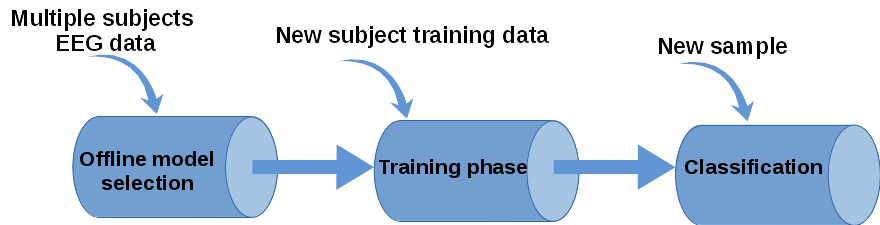
\includegraphics[width=0.8\columnwidth]{Figures/proposed-processing-pipeline.png}
\caption{Adopted machine learning pipeline. It consists of 3 main phases: 1) Offline model selection: A number of preprocessing and classifiers are tested on a collection of data from multiple subjects, the best combination is selected. 2) Training phase: Classifier parameters are trained for each new subject before classification. 3) Classification: A new [unseen] sample is preprocessed similarly to training data, then classified.}
\label{fig:porposed-pipeline}
\end{figure}  